\subsubsection{Eliminar Registro de Vehículo}
En la siguiente imagen \ref{fig:Diagrama de Secuencia - Eliminar Entrada de Vehículo}, se muestra el diagrama de secuencia correspondiente a la eliminación de algún registro para darle 'salida' al vehículo que se ha reparado. El sistema muestra un 'mensaje de seguridad' para verificar al usuario si esta seguro de borrar ese registro de la base de datos. Es en este punto donde el sistema toma dos caminos:
\begin{itemize}
	\item \textbf{Aceptación:} El Mecánico (usuario) acepta que desea eliminar ese registro, el sistema solicita a la base de datos la eliminación de dicho registro.
	\item \textbf{Cancelación:} Se elige la opción 'Cancelar' en la interfaz de usuario, el sistema desaparece el 'mensaje de seguridad' y la base de datos queda intacta. 
\end{itemize}
\begin{figure}[!h]
	\centering
	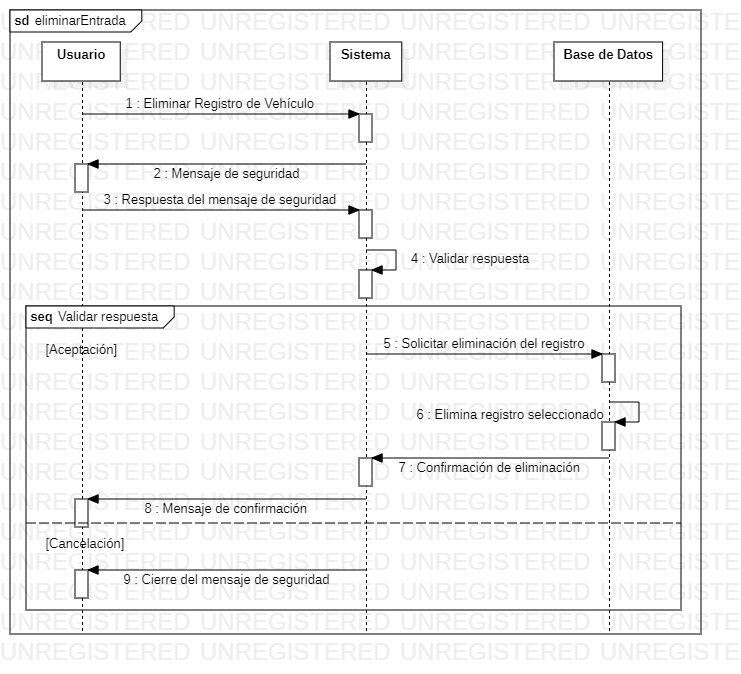
\includegraphics[width=0.9\textwidth]{./diseno/vprocesos/imagenes/eliminarEntrada}
	\caption{Diagrama de Secuencia - Eliminar Entrada de Vehículo}
	\label{fig:Diagrama de Secuencia - Eliminar Entrada de Vehículo}
\end{figure}
\clearpage